% documentclass options:
\documentclass[11pt,
  a4paper,
  parskip=half, % This is some extra vertical space between paragraphs, the suggestion is 2cm which is really ugly, so we use what koma script gives us
  % you can also set it to full for even more space. But there is a bad tex style decision: parskip also changes the spacing between listitems such as
  % enumerate and itemize. For this purpose we include the enumitem package and set itemsep=.5em, of course you can change this
  BCOR=-5mm, % BCOR is binding correction
  english,
  % if you'd rather have a one sided thesis, add `oneside' to the documentclass
  oneside,
  % ngerman is needed for hyphenation if the thesis contains parts written in German, switch order with english if you write mainly in English.
  % Remember to change order in the babel package (below) as well.
  % Last language is the preferred one.
  ngerman]{scrbook}
\usepackage[english, ngerman]{babel} % If you write mainly in English change order to ngerman, english. Also change that in the documentclass options above.
% Include of titling must happen before \title etc.
% that's why it's not in setup.tex
\usepackage{titling}
\title{Dynamic Analysis of Message-Passing Go Programs}
\author{Erik Daniel Kassubek}

% Change to your first examiner
% The ~ enables non sentence spacing after a period
\newcommand{\firstexaminer}{Prof.~Dr.~Thiemann}
% Change to your second examiner, some undergraduate studies don't have a second examiner
% in this case just comment out the following line
% \newcommand{\secondexaminer}{Prof.~Dr.~Wile E. Coyote}
% Change to your advisers
\newcommand{\advisers}{Prof.~Dr.~Thiemann\\Prof.~Dr.~Sulzmann}

% include all packages and define commands in setup.tex

%------------------------------------------------------------------------------
%       package includes
%------------------------------------------------------------------------------
    % font encoding is set up for pdflatex, for other environments see
    % http://tex.stackexchange.com/questions/44694/fontenc-vs-inputenc
    \usepackage[T1]{fontenc}  % 8-bit fonts, improves handling of hyphenations
    % provides `old' commands for table of contents. Eases the ability to switch
    % between book and scrbook
    \usepackage{scrhack}


    % ------------------- layout, default -------------------
    % adjust the style of float's captions, separated from text to improve readabilty
    \usepackage[labelfont=bf, labelsep=colon, format=hang, textfont=singlespacing]{caption}
    % With format = hang your caption will look like this:
    % Figure 1: Lorem ipsum dolor sit amet,
    %           consectetuer adipiscing elit.
    %           Ut purus elit, vestibulum
    % If you instead want
    % Figure 1: Lorem ipsum dolor sit amet,
    % consectetuer adipiscing elit. Ut purus
    % elit, vestibulum
    % change to format=plain
    \usepackage{chngcntr}  % continuous numbering of figures/tables over chapters
    \counterwithout{equation}{chapter}
    \counterwithout{figure}{chapter}
    \counterwithout{table}{chapter}
    \captionsetup{%
      figurename=Abb.,
      tablename=Tab.
   }
    

    % Uncomment the following line if you switch from scrbook to book
    % and comment the setkomafont line
    %\usepackage{titlesec}  % remove "Chapter" from the chapter title
    %\titleformat{\chapter}[hang]{\bfseries\huge}{\thechapter}{2pc}{\huge}
    \setkomafont{chapter}{\normalfont\bfseries\huge}

    \usepackage{setspace}  % Line spacing
    \onehalfspacing
    % \doublespacing  % uncomment for double spacing, e.g. for annotations in correction

    % ------------------- functional, default-------------------
    \usepackage[dvipsnames]{xcolor}  % more colors
    \usepackage{array}  % custom format per column in table - needed on the title page
    \usepackage{graphicx}  % include graphics
    \usepackage{subfig}  % divide figure, e.g. 1(a), 1(b)...
    \usepackage{amsmath}  % |
    \usepackage{amsthm}   % | math, bmatrix etc
    \usepackage{mathtools} % |
    \usepackage{amsfonts} % |
    \usepackage{amssymb}
    \usepackage{nicefrac}
    \usepackage{calc}  % calculate within LaTeX
    \usepackage[unicode=true,bookmarks=true,bookmarksnumbered=true,
                bookmarksopen=true,bookmarksopenlevel=1,breaklinks=false,
                pdfborder={0 0 0},backref=false,colorlinks=false]{hyperref}
    \usepackage{etoolbox} % if-else commands


    %==========================================
    % You might not need the following packages, I only included them as they
    % are needed for the example floats
    % ------------------- functional, custom -------------------
    \usepackage{algorithm,algpseudocode}
    \usepackage{bm}  % bold greek variables (boldmath)
    \usepackage{tikz}
    \usetikzlibrary{positioning}  % use: above left of, etc
    
    % Required for the ToDo list.
    \usepackage{ifthen}

    % Improves general appearance of the text
    \usepackage[protrusion=true,expansion=true, kerning]{microtype}
    \usepackage{enumitem}
    % Nicer font for pdf rendering.
    %\usepackage{lmodern}
    
    % For nicer looking tables.
    \usepackage{booktabs}

    % You don't need this, just for demonstration of a longer caption.
    \usepackage{lipsum}

%------------------------------------------------------------------------------
%       (re)new commands / settings
%------------------------------------------------------------------------------
    % ----------------- referencing ----------------
    \newcommand{\secref}[1]{Section~\ref{#1}}
    \newcommand{\chapref}[1]{Chapter~\ref{#1}}
    \renewcommand{\eqref}[1]{Equation~(\ref{#1})}
    \newcommand{\figref}[1]{Figure~\ref{#1}}
    \newcommand{\tabref}[1]{Table~\ref{#1}}

    % ------------------- colors -------------------
    \definecolor{darkgreen}{rgb}{0.0, 0.5, 0.0}
    % Colors of the Albert Ludwigs University as in
    % https://www.zuv.uni-freiburg.de/service/cd/cd-manual/farbwelt
    \definecolor{UniBlue}{RGB}{0, 74, 153}
    \definecolor{UniRed}{RGB}{193, 0, 42}
    \definecolor{UniGrey}{RGB}{154, 155, 156}


    % ------------------- layout -------------------
    % prevents floating objects from being placed ahead of their section
    \let\mySection\section\renewcommand{\section}{\suppressfloats[t]\mySection}
    \let\mySubSection\subsection\renewcommand{\subsection}{\suppressfloats[t]\mySubSection}


    % -------------------- others -------------------
    \usepackage{makecell}

    % ------------------- math formatting commands -------------------
    % define vectors to be bold instead of using an arrow
    \renewcommand{\vec}[1]{\mathbf{#1}}
    \newcommand{\mat}[1]{\mathbf{#1}}
    % tag equation with name
    \newcommand{\eqname}[1]{\tag*{#1}}


    % ------------------- pdf settings -------------------
    % ADAPT THIS
    \hypersetup{pdftitle={\thetitle},
                pdfauthor={\theauthor},
                pdfsubject={Undergraduate thesis at the Albert Ludwig University of Freiburg},
                pdfkeywords={deep learning, awesome algorithm,  undergraduate thesis},
                pdfpagelayout=OneColumn, pdfnewwindow=true, pdfstartview=XYZ, plainpages=false}


    %==========================================
    % You might not need the following commands, I only included them as they
    % are needed for the example floats

    % ------------------- Tikz styles -------------------
    \tikzset{>=latex}  % arrow style


    % ------------------- algorithm ---------------------
    \usepackage{listings}
    \lstset{
    frame=single,
    basicstyle=\footnotesize,
    % keywordstyle=\color{red},
    numbers=left,
    numbersep=5pt,
    showstringspaces=false, 
    % stringstyle=\color{blue},
    tabsize=2,
    language=Go,
    captionpos=b,
    linewidth=\textwidth,
    xleftmargin=0.2\textwidth,
    xrightmargin=0.2\textwidth
}

    % Command to align comments in algorithm
    \newcommand{\alignedComment}[1]{\Comment{\parbox[t]{.35\linewidth}{#1}}}
    % define a foreach command in algorithms
    \algnewcommand\algorithmicforeach{\textbf{foreach}}
    \algdef{S}[FOR]{ForEach}[1]{\algorithmicforeach\ #1\ \algorithmicdo}

    % line spacing should be 1.5
    \renewcommand{\baselinestretch}{1.5}

    % set distance between items in a list, for more details see the
    % enumitem package: https://www.ctan.org/pkg/enumitem
    \setlist{itemsep=0em}
    
    % use ra in your tables to increase the space between rows
    % 1.3 should be fine
    \newcommand{\ra}[1]{\renewcommand{\arraystretch}{#1}}

	% ToDo counters
	\usepackage{ifthen} %für whiledo-Schleife
	\newcounter{todos}
	\setcounter{todos}{0}
	\newcounter{extends}
	\setcounter{extends}{0}
	\newcounter{drafts}
	\setcounter{drafts}{0}

	% ------------------- marker commands -------------------
    % ToDo command
    \newcommand{\todo}[1]{\textbf{\textcolor{red}{(TODO: #1)}}\refstepcounter{todos}\label{todo \thetodos}}
	\newcommand{\extend}[1]{\textbf{\textcolor{darkgreen}{(EXTEND: #1)}}\refstepcounter{extends}\label{extend \theextends}}
	% Lighter color to note down quick drafts
	\newcommand{\draft}[1]{\textbf{\textcolor{NavyBlue}{(DRAFT: #1)}}\refstepcounter{drafts}\label{draft \thedrafts}}
	
	% microtype with lmodern, see https://tex.stackexchange.com/questions/75305/microtype-warning-with-lmodern-package-and-koma-script
	%\DeclareMicrotypeAlias{lmss}{cmr}

% ---------------- other --------------------



\begin{document}
    \pagestyle{empty} % no header and no page number
    % disable hyper links to remove warning "destination with same identifier"
    % this means within this section nothing can be referenced with a hyperlink
    \hypersetup{pageanchor=false}

    % enable/disable, depending on your chosen language
    \begin{titlepage}
\begin{center}

\newcommand{\HorizontalLine}{\rule{\linewidth}{0.3mm}}

{\Large Bachelorarbeit}\\[1.3cm]


% _____________________________________________________________________________
\HorizontalLine\\[0.4cm]
% Write your title in a fancy way like this if you want to customize it, otherwise simply let tex do it for you
% \begin{spacing}{3}
%     {\huge \bfseries Der Lange, Lange } \\
%     {\huge \bfseries Lange Lange} \\
%     {\huge \bfseries Titel}\\
% \end{spacing}
{ \huge \bfseries \thetitle}
\HorizontalLine\\[1.5cm]
% _____________________________________________________________________________


{\Huge \theauthor} \\[2cm]


\begin{tabular}[hc]{>{\huge}l >{\huge}l}
  Gutachter: & \firstexaminer\\[0.3cm]
  Betreuer: & \makecell[t]{\advisers}\\[1.2cm]
\end{tabular}
\vfill  % move the following text to the bottom

\Large {
    Albert-Ludwigs-Universität Freiburg\\
    Technische Fakultät\\
    Institut für Informatik\\[1cm]

    14. Februar 2023
    \\
}
\end{center}
\end{titlepage}

\thispagestyle{empty}
% title page back
\ \vfill \ \\  % at least one space required before vfill
\
\textbf{Bearbeitungszeit}            \smallskip{} \\
14.\,11.\,2022 -- 14.\,02.\,2023   \bigskip{} \\
\
\textbf{Gutachter}                  \smallskip{} \\
\firstexaminer                      \bigskip{} \\
\
% If there is a second examiner include it
\ifdef{\secondexaminer}
	{
	% Include
	\textbf{Zweitgutachter}        \smallskip{} \\
	\secondexaminer               \bigskip{} \\
	\
	}
	{
	% No second examiner, ignore
	}
\textbf{Betreuer}                  \smallskip{} \\
\advisers

    \pagestyle{plain} % remove chapter name from top, page number at the bottom
    % use \pagestyle{headings} for having the chapter on top of the pages
    % if you want a more fancy header use \usepackage[automark,headsepline]{scrlayer-scrpage}
    % and read about it in the KOMA script documentation, https://www.ctan.org/pkg/koma-script
    \frontmatter  % roman page numbers
    % Copied from the official declaration from the examination office (typos fixed).
% Please double check the wording on their website and report changes.
% (https://www.tf.uni-freiburg.de/de/studium-lehre/a-bis-z-studium/dokumente/Declarationforthefinalthesis.pdf)

\chapter*{ERKLÄRUNG}
Hiermit erkläre ich, dass ich diese Abschlussarbeit selbständig verfasst habe, keine anderen
als die angegebenen Quellen/Hilfsmittel verwendet habe und alle Stellen, die wörtlich oder
sinngemäß aus veröffentlichten Schriften entnommen wurden, als solche kenntlich gemacht
habe. Darüber hinaus erkläre ich, dass diese Abschlussarbeit nicht, auch nicht
auszugsweise, bereits für eine andere Prüfung angefertigt wurde.
\\[3\normalbaselineskip]
\begin{tabular}{p{\textwidth/2} l}
  \rule{\textwidth/3}{0.4pt}   &   \rule{\textwidth/3}{0.4pt} \\
  Ort, Datum                  &   Unterschrift
\end{tabular}

    \chapter*{Zusammenfassung}
Go ist eine Programmiersprache, welche einen besonderen Fokus auf 
die Erzeugung von effizienten nebenläufigen Programmen legt. Dazu 
stellt Go s.g. Go-Routinen als leichtgewichtige Threads sowie 
Mutexe und Channels zur Synchronisation von und Kommunikation zwischen 
solchen Routinen bereit. Solche Konstrukte können aber leicht zu 
Concurrency-Bugs führen, welche auf Grund ihre starken Abhängigkeit von der 
genauen Ausführung des Programms nur schwer erkennbar sind.\\
Diese Arbeit entwickelt und implementiert einen dynamischen Detektor zur
Erkennung solcher Probleme. Der Detektor verbindet dabei die Detektion 
von Bugs durch Mutexe mit Lock-Bäumen, sowie die Betrachtung von 
Bugs auf Channels, sowie deren potenzielle Kommunikationspartner mit Hilfe von 
Vector-Clocks. Außerdem ist der Detektor in der 
Lage mehrere, durch Select-Statement verzweigte Ausführungspfade zu betrachten.
    \tableofcontents
    \hypersetup{pageanchor=true}  % re-enable hyperlinking

    \mainmatter % Arabic page numbers
    \chapter{Einführung}\label{chap:introduction}
Go ist eine seit 2007 von Google entwickelte Programmiersprache, welche sich 
in den letzten Jahren zu einer der beliebtesten Programmiersprachen entwickelt 
hat~\cite{ranking}. Ein Fokus der Sprache liegt dabei auf der Erstellung
sicherer und effizienter nebenläufiger Programme. Go stellt verschiedene 
Funktionen für die Erstellung solcher nebenläufiger Programme zur Verfügung.
Die wichtigsten sind dieser Funktionen sind dabei Go-Routinen, Mutexe und 
Channels.\\Go-Routinen erlauben das nebenläufige Ausführen mehrerer Codeteile.
Mutexe erlauben die Synchronisation von Routinen, sowie die Lösung des Problems 
des kritischen Ausschlusses. 
Channel können ebenfalls für die Synchronisation verwendet werden,
können aber zusätzlich für eine Kommunikation, bzw.\ das Senden von Daten zwischen 
Routinen verwendet werden. Programmierer werden dabei angehalten, Channel
anstelle von gemeinsamen Variablen zu verwenden, da bei diesen die Wahrscheinlichkeit
für das Auftreten von Concurrency-Bugs geringer ist~\cite{sharedMemory}.\\
Solche Bugs (z.B. Deadlocks), welche durch die Nebenläufigkeit von Programmen sowie ihrer 
Synchronisationsmechanismen entstehen sind in der Praxis aber dennoch sehr weit 
verbreitet~\cite{numberBugs}.\\\\
Diese Arbeit beschäftigt sich mit der Entwicklung und Implementierung
eines dynamischen Detektors ``GoChan'' für die automatische Erkennung
von Problemen, welche durch die Verwendung von Mutexen und Channels 
in nebenläufigen Go-Programmen entstehen. Der größte Fokus wird dabei 
auf die Erkennung und Analyse von Deadlock-Situationen, sowie das vorzeitige 
schließen von Channels gelegt, da diese zu einem Absturz eines Programms 
führen können. Der Detektor vereinigt dabei verschiedene Methoden aus 
iGoodLock~\cite{iGoodLock} und UNDEAD~\cite{Undead} sowie 
Gopherlyzer-GoScout~\cite{PPDP18} und GFuzz~\cite{gfuzz} zur 
Erkennung und Analyse von 
durch Mutenxen und Channels erzeugten Bugs.\\
GoChan basiert dabei aus zwei Programmen, einem Instrumenter und einem 
Analyzer, für welche jeweils eine 
Implementierung vorliegt. Für die Analyze wird das zu analysierende Programm 
mehrfach durchlaufen. Bei jedem Durchlauf zeichnet der Analyzer relevante 
Situationen auf und führt anschließend, basieren auf dem so erstellten Trace 
eine Analyse aus, um Probleme zu erkennen. Die Analyse wird mehrfach wiederholt, 
um verschiedene Ausführungspfade zu analysiere, welche durch die Verwendung 
verschiedener Pfade in Select-Operationen erzeugt werden. Um den Trace eines 
Programmdurchlaufs aufzeichnen zu können und bei Select-Operationen verschiedene 
Ausführungspfade zu erzwingen, muss der zu analysierende Programmcode 
verändert werden. Dies kann durch den Instrumenter automatisiert erfolgen.\\\\
Der Aufbau dieser Arbeit ist wie folgt. Zuerst wird in Abschnitt~\ref{chap:background}
die theoretische Funktionsweise des Detektors beschrieben und dargelegt, 
welche Art von Situationen der Detektor erkennen soll. 
Abschnitt~\ref{Chap:Instrumenter} geht auf die Funktionsweise und Implementierung 
des Instrumenters und Abschnitt~\ref{Chap:Implement} auf die Implementierung 
des Analyzers ein. In Abschnitt~\ref{Chap:Eval} wird der Detektor auf 
konstruierte und tatsächliche Programme angewandt, um zu überprüfen, 
wie gut er in der Lage ist, Probleme richtig einzusätzen. Für die 
tatsächlichen Programme werden dabei Programme aus GoBench~\cite{gobench}
verwendet, welche eine Sammlung von Programmen mit Concurrency-Bugs aus 
mehreren großen open-source Programmen besitzt. Zuletzt werden die 
Erkenntnisse in Abschnitt~\ref{chap:conclusion} zusammengefasst. Die Implementierung
der beschriebenen Programme befindet sich in \url{https://github.com/ErikKassubek/GoChan}.

    \chapter{Hintergrund}\label{chap:background}
% \draft{Hintergrund Einführung}\\
% Es gibt bereits Methoden zur Erkennung von Concurrency-Bugs in
% Go Programmen, in denen Nachrichten zwischen Routinen ausgetauscht werden. 

% Im folgenden sollen zwei solche Methoden betrachtet und verglichen werden. 
% Dabei handelt es sich um ``Two-Phase Dynamic Analysis of Message-Passing Go
% Programs based on Vector Clocks'' von Sulzmann und Stadtmüller~\cite{PPDP18}
% und ``Who Goes First? Detecting Go Concurrency Bugs via Message Reordering'' 
% von Liu und Xia et al.~\cite{gfuzz}.

% \section{Two-Phase Dynamic Analysis of Message-Passing Go
% Programs based on Vector Clocks}\label{sec:PPDP18}
% \todo{Beschreibung von PPDP18}\\
% \extend{Beschreibung von PPDP18}\\
% Die Analyse von Sulzmann und Stadtmüller, im folgenden kurz als PPDP18 bezeichnet,
% nutzt ein zweiphasiges Model um Vector-Clock-Informationen zu erhalten auf 
% Basis welcher im Anschluss durch Trace-Replay nach möglichen Message Contentions,
% dem Senden zu einem geschlossenen Kanal, 
% Deadlock Recovery und alternativen 
% Kommunikationspartnern für Send/Receive Paare gesucht wird.

% \subsection{Tracing}\label{subsec:PPDP18Tracing}
% Mit dem Tracing wird der Ablauf eines Programmdurchlaufs aufgezeichnet. Aus 
% diesen Aufzeichnungen lassen sich im Anschluss die Vector-Clocks ableiten.
% Die Events werden dabei für jede Routinen einzeln aufgezeichnet. Für das 
% Senden und Empfangen über Channels werden jeweils ein Pre- und ein Postevent
% gespeichert.\\
% Im einzelnen werden die folgenden Events gespeichert:
% \begin{itemize}
%   \item $signal(i), wait(i)$ speichern das Erzeugen einer neuen Routinen.
%   \item $pre(x?), pre(x!)$ werden gespeichert, bevor Channel $x$ versucht eine Nachrichten zu erhalten oder zu senden.
%   \item $post(i, j, x?), pos(i, j, x!)$ werden gespeichert, wenn die Übertragung einer Nachricht über den Channel $x$ erfolgreich abgeschlossen 
%         worden ist. Dabei wird außerdem die ID des Kommunikationspartners $i$, sowie ein Zeitstempel $j$ der sendenden Routine aufgezeichnet.
%   \item $close(x)$ zeichnet auf, dass Channel $x$ geschlossen speichert.
%   \item $post(default)$ wird in dem Trace gespeichert, wenn der Default-Case in einem Switch-Statement ausgeführt wurde.
% \end{itemize}
% Man betrachte das folgende Beispielprogramm. Die Hauptroutine sei dabei Routine 1.
% Alle anderen Routinen sind mit ihrer ID versehen.
% \lstinputlisting{code/02-background/example_trace.txt}
% Der resultierende Trace gibt sich dabei zu 
% \begin{align*}
%   [&1\#[signal(2), signal(3), signal(4), signal(5)],\\
%    &2\#[wait(2), pre(x!), post(2, 1, x!)],\\
%    &3\#[wait(3), pre(x?), post(2, 1, x?), pre(x!), post(3, 2, x!)],\\
%    &4\#[wait(4), pre(y!), post(4, 1, y!), pre(x?), post(3, 2, x?)],\\
%    &5\#[wait(5), pre(y?), post(4, 1, y?)]]\\
% \end{align*}
   
    \chapter{Tracer}\label{Chap:Tracer}
Um ein Program analysieren zu können, wird der Ablauf eines Programmdurchlaufs
aufgezeichnet. Dazu wurde ein Tracer implementiert, durch welchem die 
Channel- und Lock-Operationen, sowie andere Operationen wie Select und das 
erzeugen einer neuen Routine, ersetzt, bzw. erweitert werden. Diese 
führen die eigentlichen Operationen aus und zeichnen gleichzeitig den 
Trace auf. Die Ersetzung durch die Drop-In Replacements kann dabei automatisch 
durch einen Instrumenter erfolgen, welche mit Hilfe des Abstract Syntax Tress 
die Ersetzungen vornimmt.\\
Anders als in vielen anderen Programmen, welche den Trace von Go-Programmen
analysieren, wie z.B.~\cite{GoAt2} oder~\cite{GoVis} wird dabei der Tracer 
selbst implementiert und basiert nicht auf dem Go-Runtime-Tracer~\cite{GoRunTrace}. 
Dies ermöglicht es, den Tracer genau auf die benötigten Informationen zuzuschneiden
und so einen geringeren negativen Einfluss auf die Laufzeit des Programms zu erreichen.

\extend{Tracer Einführung}

\section{Trace}\label{Chap:Tracer-Sec:Trace}
\draft{Trace} 
Der Aufbau des Trace basiert auf~\cite{PPDP18}. Er wird aber um Informationen 
über Locks erweitert. Der Trace wird für jede Routine
separat aufgezeichnet. Außerdem wird, anders als in~\cite{PPDP18} ein globaler
Program-Counter für alle Routinen und nicht ein separater Counter für jede 
Routine verwendet. Dies ermöglicht es bessere Rückschlüsse über den genauen 
Ablauf des Programms zu ziehen.  
Die Syntax des Traces in EBNF gibt sich 
folgendermaßen:
\begin{align*}
  \begin{matrix*}[l]
    T & = & ''\ [\ '',\ \{\ U\ \},\ ''\ ]\ ''; & \text{Trace}\\
    U & = & ''\ [\ '',\ \{\ t\ \},\ ''\ ]\ ''; & \text{lokaler Trace} \\
    t & = & signal(t, i)\ |\ wait(t, i)\ |\ pre(t, as)\ |\ post(t, i, x!) & \text{Event}\\
      &   & |\ post(t, i, x?, t') |\ post(t, default)\ |\ close(t, x)\  & \\
      &   & |\ lock(t, y, b, c) |\ unlock(t, y); & \\
    a & = & x,\ (''\ !\ ''\ |\ ''\ ?\ ''); & \\
    as & = & a\ |\ (\{\ a\ \}, [\ ''\ default\ ''\ ]); & \\
    b & = & ''-''\ |\ ''t''\ |\ ''r''\ |\ ''tr'' & \\
    c & = & ''0''\ |\ ''1''
  \end{matrix*}
\end{align*}
wobei $i$ die Id einer Routine, $t$ einen globalen Zeitstempel, $x$ die Id eines 
Channels und $y$ die Id eines Locks darstellt. Die Events haben dabei folgende Bedeutung:
\begin{itemize}
  \item \texttt{signal(t, i)}: In der momentanen Routine wurde
    eine Fork-Operation ausgeführt,
    d.h. eine neue Routine mit Id $i$ wurde erzeugt.
  \item \texttt{wait(t, i)}: Die momentane Routine mit Id $i$ wurde soeben erzeugt. Dies ist 
    in allen Routinen außer der Main-Routine das erste Event in ihrem lokalen Trace.
  \item \texttt{pre(t, as)}: Die Routine ist an einer Send- oder Receive-Operation eines 
    Channels oder an einem Select-Statement angekommen, dieses wurde aber noch nicht 
    ausgeführt. Das Argument $as$ gibt dabei die Richtung und den Channel an. 
    Ist $as = x!$, dann befindet sich der Trace vor einer Send-Operation, bei 
    $as = x?$ vor einer Receive-Operation. Bei einem Select-Statement ist 
    $as$ eine Liste aller Channels für die es einen 
    Case in dem Statement gibt. Besitzt das Statement einen Default-Case, wird
    dieser ebenfalls in diese List aufgenommen.
  \item \texttt{post(t, i, x!)}: Dieses Event wird in dem Trace gespeichert, nachdem 
    eine Send-Operation auf $x$ erfolgreich abgeschlossen wurde. 
    $i$ gibt dabei die Id der sendenden Routine
    an.
  \item \texttt{post(t, i, x?, t')}: Dieses Event wird in dem Trace gespeichert, nachdem 
    eine Receive-Operation des Channels $x$ erfolgreich abgeschlossen wurde. 
    $i$ gibt dabei die Id der sendenden Routine an. $t'$ gibt den Zeitstempel an,
    welcher bei dem Pre-Event der sendenden Routine galt. Durch die Speicherung der Id und des 
    Zeitstempels der sendenden Routine bei einer Receive-Operation lassen sich 
    die Send- und Receive-Operationen eindeutig zueinander zuordnen.
  \item \texttt{post(t, default)}: Wird in einem Select-Statement der Default-Case ausgeführt,
    wird dies in dem Trace der entsprechenden Routine durch $post(t, default)$ 
    gespeichert.
  \item \texttt{close(t, x)}: Mit diesem Eintrag wird das schließen eines Channels $x$ 
    in dem Trace aufgezeichnet.
  \item \texttt{lock(t, y, b, c)}: Der Beanspruchungsversuch eines Locks mit id $y$ wurde beendet. 
    $b$ gibt dabei die Art der Beanspruchung an. Bei $b = r$ war es eine R-Lock
    Operation, bei $b = t$ eine Try-Lock Operation und bei $b = tr$ ein Try-R-Lock
    Operation. Bei einer normalen Lock-Operation ist $b = -$. Bei einer 
    Try-Lock Operation kann es passieren, dass die Operation beendet wird, 
    ohne das das Lock gehalten wird. In diesem Fall wird $c$ auf $0$, und 
    sonst auf $1$ gesetzt. 
  \item \texttt{unlock(t, y)}: Das Lock mit id $y$ wurde zum Zeitpunkt 
    $t$ wieder freigegeben. 
\end{itemize}
Um diesen Trace zu erzeugen, werden die Standartoperation aud Go durch Elemente
des Tracers ersetzt. Die Funktionsweisen dieser Ersetzungen sind im folgenden 
angegeben. Dabei werden nur solche Ersetzungen angegeben, welche direkt 
für die Erzeugung
des Traces notwendig sind. Zusätzlich werden noch 
weitere Ersetzungen durchgeführt, wie z.B. die Ersetzung der Erzeugung von 
Mutexen und Channel von den Standardvarianten zu den Varianten des Tracers.
Hierbei wird auch die Größe jedes Channels gespeichert.
Dies werden in der Übersicht zur Vereinfachung nicht betrachte. Auch werden 
in der Übersicht nur die Elemente betrachtet, die für die Durchführung der 
Operation und dem Aufbau des Traces benötigt werden. Hilfselemente, wie z.B. 
Mutexe, welche verhindern, dass mehrere Routinen gleichzeitig auf die selbe 
Datenstruktur, 
z.B. die Liste der Listen, welche die Traces für die einzelnen Routinen 
speichern, zugreifen, werden nicht mit angegeben. Dabei sei $c$ ein 
Zähler, $nR$ ein Zähler für die Anzahl der Routinen, $nM$ ein Zähler für die 
Anzahl der Mutexe und $nC$ ein Zähler für die Anzahl der Channels. $nM$ und $nC$
werden bei der Erzeugung eines neuen Mutex bzw. eines neuen Channels atomarisch 
Incrementiert. Den erzeugten Elementen wird er neue Wert als $id$ zugeordnet. All diese 
Zähler seien global und zu Beginn als $0$ initialisiert. Außerdem bezeichnet 
$mu$ einen Mutex, $rmu$ einen RW-Mutex, $ch$ einen Channel und $B$ bzw. $B_i$
mit $i\in\mathbb{N}$ den 
Körper einer Operation. Zusätzlich
sei $id$ die $Id$ der Routine, in der eine Operation ausgeführt wird,
$[signal(t, i)]^{id}$ bedeute, dass der das entsprechende Element (hier als 
Beispiel $signal(t, i))$, in den Trace der Routine mit id $id$ eingeführt wird
und $[+]^i$ bedeute, das in die Liste der Traces ein neuer, leerer Trace 
eingefügt wird, welcher für die Speicherung des Traces der Routine $i$ 
verwendet wird. 
$\langle a|b\rangle$ bedeutet, dass ein Wert je nach Situation auf $a$ oder $b$ gesetzt 
wird. Welcher Wert dabei verwendet wird, ist aus der obigen Beschreibung der 
Trace-Elemente erkennbar. $\text{e}_1$ bis $\text{e}_n$ bezeichnet die Selektoren in einem Select statement.
$\text{e}_i^*$ bezeichnet dabei einen Identifier für einen Selektor, der sowohl die 
Id des beteiligten Channels beinhaltet, als auch die Information, ob es sich um ein 
Send oder Receive handelt und $\text{e}_i^m$ die Message, die in einem Case 
empfangen wurde. 
\begin{tabular}{lcl}
  go B & $\Rightarrow$ & nr := atomicInc(nR); ts := atomicInc(c); [ signal(ts, nr) ]$^\text{nr}$;\\
    & & [+]$^\text{nr}$; go \{ ts' := atomicInc(c); [ wait(ts, nr) ]$^\text{id}$; B\};\\
  ch <- i & $\Rightarrow$ & ts := atomicInc(c); [ pre(ts, ch.id, true) ]$^\text{id}$; ch <- \{i, id, ts\};\\
    & & ts' := atomicInc(c); [ post(ts', ch.id, true, id) ]$^\text{id}$\\
  <- ch & $\Rightarrow$ & ts := atomicInc(c); [ pre(ts, ch.id, false) ]$^\text{id}$;\\
    & & \{i, id\_send, ts\_send\} := <-c; ts' := atomicInc(c);\\
    & & [ post(ts', ch.id, false, id\_send, ts\_send) ]$^\text{id}$; return i;\\
  close(ch) & $\Rightarrow$ & ts := atomicInc(c); close(ch); [ close(ts, ch.id) ]$^\text{id}$\\
  select(e$_\text{i} \leadsto \text{B}_\text{i}$) & $\Rightarrow$ & ts := atomicInc(c); [ pre(ts, e$_1^*$, $\ldots$, e$_n^*$, false) ]$^\text{id}$;\\
    & & select(e$_\text{i} \leadsto$ \{ ts' := atomicInc(c);\\
    & & [ $\langle \text{post(ts, e$_\text{i}$.ch, false, e$_\text{i}^\text{m}$.id\_send, e$_\text{i}^\text{m}$.ts\_send)}\ |$ \\
    & & post(ts, e$_\text{i}$.ch, true, id) $\rangle$ ]$^\text{id}$ B$_\text{i}$\}) \\
  select(e$_\text{i} \leadsto \text{B}_\text{i}$ | B$_\text{def}$) & $\Rightarrow$ & ts := atomicInc(c); [ pre(ts, e$_1^*$, $\ldots$, e$_n^*$, false) ]$^\text{id}$;\\
    & & select(e$_\text{i} \leadsto$ \{ ts' := atomicInc(c);\\
    & & [ $\langle \text{post(ts, e$_\text{i}$.ch, false, e$_\text{i}^\text{m}$.id\_send, e$_\text{i}^\text{m}$.ts\_send)}\ |$ \\
    & & post(ts, e$_\text{i}$.ch, true, id) $\rangle$ ]$^\text{id}$ B$_\text{i}$\} |\\
    & & ts' := atomicInc(c); [ default(ts) ]$^\text{id}$; B$_\text{def}$) \\
  mu.(Try)Lock() & $\Rightarrow$ & ts := atomicInc(c); mu.(Try)Lock();\\
    & & [ lock(ts, mu.id, $\langle \text{-|t}\rangle$, $\langle \text{0|1}\rangle$) ]$^\text{id}$;\\
  mu.Unlock() & $\Rightarrow$ & ts := atomicInc(c); mu.Unlock(); [ unlock(ts, mu.id) ]$^\text{id}$;\\
  rmu.(Try)(R)Lock() & $\Rightarrow$ & ts := atomicInc(c); rmu.(Try)(R)Lock();\\
    & & [ lock(ts, rmu.id, $\langle \text{-|t|r|tr}\rangle$, $\langle \text{0|1}\rangle$) ]$^\text{id}$;\\
  rmu.Unlock() & $\Rightarrow$ & ts := atomicInc(c); rmu.Unlock(); [ unlock(ts, rmu.id) ]$^\text{id}$;
\end{tabular}

Man betrachte als Beispiel das folgende Programm in Go:
\begin{figure}figure
  \lstinputlisting{code/03-tracer/example_code_pre.txt}
  \caption{Beispielprogramm für Tracer}
  \label{Chap:Tracer-Sec:Trace-Fig:Example}
\end{figure}
% Erweitert man diesen mit dem Tracer, erhält man folgendes Programm:
% \lstinputlisting{code/03-tracer/example_code_post.txt}
Dieser ergibt den folgenden Trace:
\begin{align*}
  [&[signal(1, 2),\ signal(2, 3),\ signal(3, 4),\ pre(4, a?, default),\ post(5, default)]\\
  &[wait(8, 2),\ lock(9, 1, -, 1),\ pre(10, x!),\ post(16, 2, x!, 1),\ unlock(17, 1)]\\
  &[wait(11, 3),\ pre(12, y!),\ post(13, 3, y!, 1),\ pre(14, x?),\ post(15, 2, x?, 10, 1)]\\
  &[wait(6, 4),\ pre(7, y?),\ post(18, 3, y?, 12, 1)]]
\end{align*}
Aus diesem lässt sich der Ablauf des Programms vollständig rekonstruieren.
\extend{Tracer}


\section{Instrumenter}\label{Chap:Tracer-Sec:Instrumenter}
\draft{Instrumenter}
Um den Trace zu erzeugen, müssen verschiedene Operationen durch Funktionen
des Tracers ersetzt bzw. erweitert werden. Wie man an dem Beispiel 
unschwer erkennen kann, besitzt die Version mit dem Tracer einen deutlich längeren
Programmcode, was bei der Implementierung zu einer größeren Arbeitslast 
führen kann. Da sich der Tracer auch negativ auf die Laufzeit des Programms 
auswirken kann, ist es in vielen Situationen nicht erwünscht, ihn in den 
eigentlichen Release-Code einzubauen, sondern eher in eine eigenständige 
Implementierung, welche nur für den Tracer verwendet werden. Um dies zu
automatisieren wurde ein zusätzliches Programm implementiert, welches in der 
Lage ist, den Tracer in normalen Go-Code einzufügen. Die Implementierung, 
welche ebenfalls in~\cite{GoChan} zur Verfügung steht, arbeitet mit einem 
Abstract Syntax Tree. Bei dem Durchlaufen dieses Baums werden die 
entsprechenden Operationen in dem Programm erkannt, und durch ihre entsprechenden 
Tracer-Funktionen ersetzt bzw.\ ergänzt. Neben dem Ersetzen der verschiedenen 
Operationen werden außerdem einige Funktionen hinzugefügt. Zu Begin der 
Main-Funktion des Programms wird der Tracer initialisiert. Zusätzlich
wird eine zusätzliche Go-Routine gestartet, in welcher ein Timer läuft. 
Ist dieser abgelaufen, wird  die Analyse gestartet, 
auch wenn das Programm noch nicht vollständig durchlaufen ist. Dies führt dazu,
dass auch Programme, in welchen ein Deadlock aufgetreten ist, analysiert 
werden können. Endet das Programm in der vorgegebenen Zeit, wird der Analyzer 
nach der Beendigung des Programms gestartet.
\extend{Instrumenter}

\section{Laufzeit}\label{Chap:Tracer-Sec:Laufzeit}
\paragraph{Instrumenter} Zuerst soll die Laufzeit des Instrumenters betrachtet 
werden. Es ist erwartbar, 
dass sich die Laufzeit linear in der Anzahl der Ersetzungen in dem AST, also 
der Anzahl der Mutex- und Channel-Operationen verhält. Dies bestätigt sich auch durch 
die Messung der Laufzeit des Programms (vgl. 
Abb.~\ref{Chap:Tracer-Sec:Laufzeit-Img:LaufzeitInstrumenter})\\
\begin{minipage}{0.45\textwidth}
  \centering  
  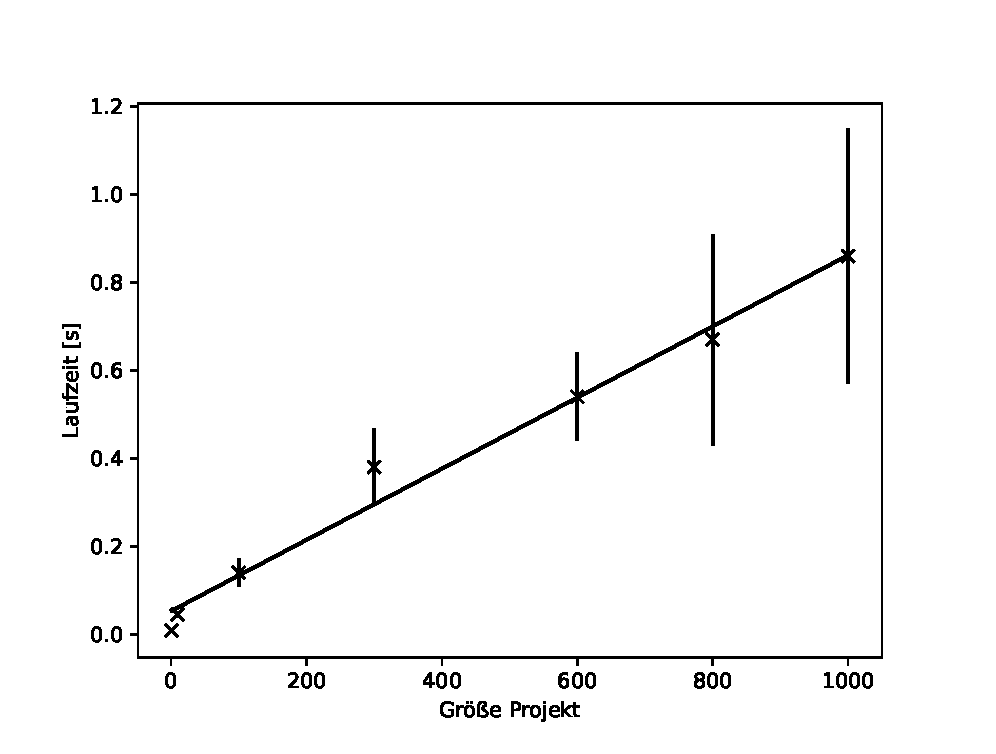
\includegraphics[width=\textwidth]{img/tracer/Runtime_Instrumenter.eps}
  \captionof{figure}{Laufzeit des Instrumenters}
  \label{Chap:Tracer-Sec:Laufzeit-Img:LaufzeitInstrumenter}
\end{minipage}
\hfill
\begin{minipage}{0.45\textwidth}
  \centering
  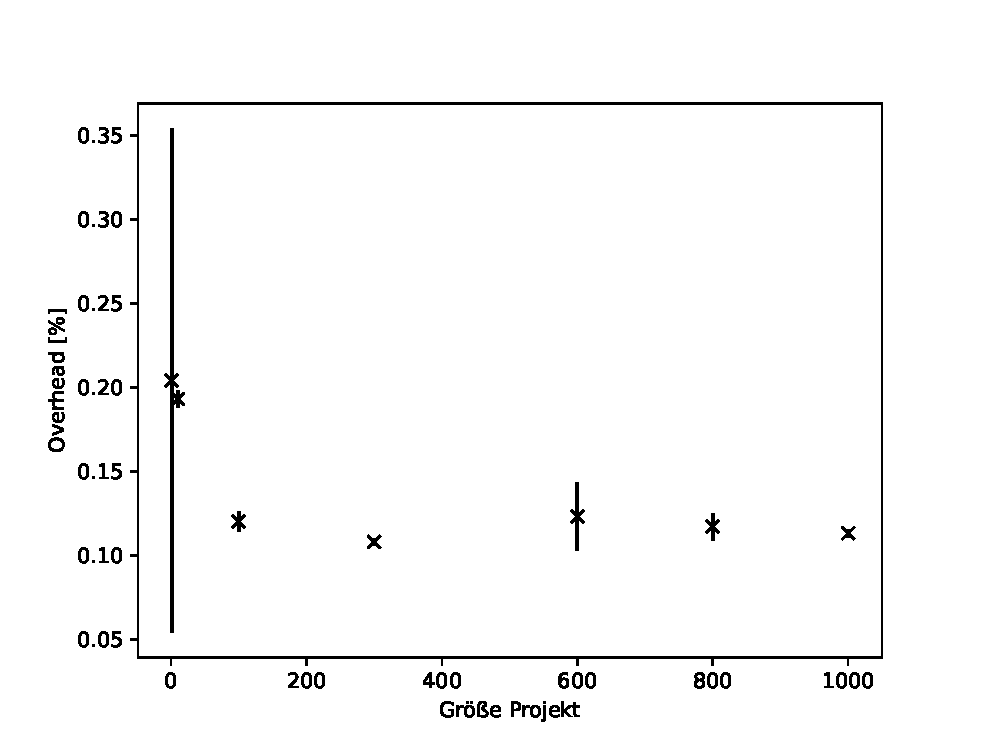
\includegraphics[width=\textwidth]{img/tracer/Runtime_Tracer.eps}
  \captionof{figure}{Prozentualer Overhead des Tracers ohne Analyse}
  \label{Chap:Trace-Sec:Laufzeit-Img:LaufzeitTracer}
\end{minipage}
Der abgebildete Graph zeigt die Laufzeit des Programms in $s$ abhängig von der 
Größe des Programms. Das Programm besteht dabei aus einem Testprogramm, welches 
alle möglichen Situationen mit Channels und Mutexen abbildet. Die Vergrößerung 
des Programmes wurde dadurch erreicht, dass die Datei mit dem Programmcode 
mehrfach in dem Projekt vorkam. Ein Projekt mit Größe $n$ besteht vor der 
Instrumentierung also 
aus $n$ Dateien, mit insgesamt $65n$ Zeilen von Code und $52n$ Ersetzungen
in dem AST. Die tatsächliche Laufzeit des Instrumenters auf einen 
Programm hängt schlussendlich natürlich von der tatsächlichen Größe des 
Projekt und der Verteilung der Mutex- und Channel-Operationen in dem Code ab.\\
\begin{table}[!h]
  \centering
  \begin{tabular}{|c|c|c|c|c|}
  \hline
  Projekt & LOC & Nr. Dateien & Nr. Ersetzungen & Zeit {[}s{]} \\ \hline
  ht-cat & $733$ & $7$ & $233$ & $0.013 \pm 0.006$ \\ \hline
  go-dsp & $2229$ & $18$ & $600$ & $0.029 \pm 0.009$ \\ \hline
  goker & $9783$ & $103$ & $4928$ & $0.09 \pm 0.03$ \\ \hline
  \end{tabular}
  \caption{Laufzeit des Instrumenters für ausgewählte Programme}
  \label{Chap:Tracer-Sec:Laufzeit-Tab:LaufzeitInstrumenter}
\end{table}
Zusätzlich wurde die Messung auch mit drei tatsächlichen Programmen 
durchgeführt. Die dort gemessenen Werte befinden sich in 
Tabelle~\ref{Chap:Tracer-Sec:Laufzeit-Tab:LaufzeitInstrumenter}. Gerade in 
Abhängigkeit von der Anzahl der Ersetzungen, stimmen die hier gemessenen Werte
mit denen in Abb.~\ref{Chap:Tracer-Sec:Laufzeit-Img:LaufzeitInstrumenter} gut 
überein, während es bei den anderen Parametern größere Abweichungen gibt.
Dies bestätigt dass der dominante Faktor für die Laufzeit des Programms 
die Anzahl der Ersetzungen in dem AST ist, und die Laufzeit linear von dieser 
abhängt.
\paragraph{Tracer} Folgend soll nun auch die Laufzeit des Tracers betrachtet werden.
Hierbei wird nur die Laufzeit des eigentlichen Tracers, nicht aber der anschließenden 
Analyse betrachtet. Um den Overhead in Abhängigkeit von der Größe des Projektes messen 
zu können, wird das selbe Testprogramm betrachtet, welches bereits in der Messung 
für den Instrumenter verwendet wurde. Abb. \ref{Chap:Trace-Sec:Laufzeit-Img:LaufzeitTracer}
zeigt den gemessenen Overhead. Der durchschnittliche Overhead über alle gemessenen Werte 
liegt dabei bei $14 \pm 2\ \%$. Da der Overhead aber linear davon abhängt, 
wie größ der Anteil der Mutex- und Channel-Operationen im Verhältniss zu 
der Größe bzw. der Laufzeit des gesammten Programms ist, kann dieser Wert abhängig 
von dem tatsächlichen Programm start schwanken. Dies wird unteranderem klar, wenn man 
den Overhead für ht-cat ($9 \pm 3\ \%$) und go-dsp ($60\pm 18\ \%$) welche $51 \pm 21$ 
Prozentpunkte außeinander liegen. 
\extend{Laufzeit}



    \chapter{Analyze}\label{Chap:Analyze}
Das folgende Kapitel soll sich nun mit der Analyze des in Kap~\ref{Chap:Tracer} erstellten 
Trace befassen. Sie befasst sich dabei mit der erkennung potentieller Deadlocks 
durch die vorkommenden Mutexe und Routinen. \extend{Mehr zur Einführung}

\section{Deadlock durch Mutext}\label{Chan:Analyze-Sec:Mutex}
\draft{Deadlock Mutex Draft}
Als erstes sollen Deadlocks betrachtet werden, welche nur von (RW-)Mutexen erzeugt werden.
Dabei wird vor allem zyklischen Locking betrachtet, bei dem sich mehrere Routinen 
gegenseitig blockieren. 
Abb.~\ref{Chap:Analyze-Sec:Mutex-Fig:Zyclic} zeigt ein Beispiel, in welchem es zu zyklischem 
Locking kommen kann.
\begin{figure}[h!]
  \lstinputlisting{code/04-analyzer/zyclic-locking-example.txt}
  \caption{Beispielprogramm zyklisches Locking}
  \label{Chap:Analyze-Sec:Mutex-Fig:Zyclic}
\end{figure}
Routine 0 und Routine 1 können dabei gleichzeitig ausgeführt werden. Man betrachte den Fall, in dem 
Zeile 7 und 14 gleichzeitig ausgeführt werden, also Lock \texttt{y} von Routine 0 und Lock \texttt{x} 
von Routine 1 gehalten wird. In diesem Fall kann in keiner der Routinen die nächste Zeile augeführt werden,
da das jeweilige Locks, welches beansprucht werden soll bereits durch die andere Routine gehalten wird. 
Da sich diese Situation auch nicht von alleine auflößen kann, blockiert dass Programm, befindet sich also 
in einem zyklischen Deadlock.\\\\
Da solche Situtationen nur in ganz besonderen Situation auftreten (in dem obigen Beispiel müssen Zeilen 
7 und 14 genau gleichzeitig ausgeführt werden, ohne dass Zeile 8 oder 15 ausgeführt werden), muss 
ein Detektor, welcher vor solchen Situationen warnen soll, nicht nur tatsächliche Deadlocks, sondern
vor allem potenzielle, also nicht tatsächlich aufgetretene Deadlocks erkenne. Die Erkennung der 
potenziellen Deadlocks basiert hierbei auf iGoodLock~\cite{iGoodLock} und UNDEAD~\cite{Undead}. Dabei wird ein Lockgraph 
aufgebaut. Dieser Speichert die in dem Programm vorkommenden Knoten, sowie ihre Abhängigkeiten. 
Dies bedeutet, dass die Knoten des Graphen gerade die (RW-)Locks representieren. Es gibt dabei 
genau dann eine Kante von Knoten \texttt{x} nach \texttt{y}, wenn das Lock \texttt{y} beansprucht 
wird, während das Lock \texttt{x} gerade von der selben Routine gehalten wird. Eine 
genauere Erklärung der Implemenierung des Locks findet sich in~\cite{bachelor-project}. \todo{ist des erlabut, oder soll ich es nochmal komplett beschreiben}  \\\\
Der Graph wird basierend auf dem zufgezeichneten Trace aufgebaut. Dazu werden die Traces der 
einzelnen Routinen nacheinander durchlaufen. Für jede Routine erzeugen wir eine Liste \texttt{currentLocks} aller 
Locks, die momentan von der Routine gehalten werden. Die einzelnen Elemente des Trace einer 
Routine werden nun durchlaufen. Handelt es sich dabei um ein Lock Event eines Locks \texttt{x}, wird 
für jedes Lock \texttt{l} in \texttt{currentLocks} eine Kante von \texttt{l} nach \texttt{x} in den 
Lock-Graphen eingefügt. Anschließend wird \texttt{x} in \texttt{currentLocks} eingefügt.
Ist das handelt es sich bei dem Element um ein unlock Event auf dem Lock \texttt{x}, dann wird das 
letzt vorkommen von \texttt{x} auf \texttt{currentLocks} entfernt.\\
Nachdem der Trace einer Routine durchlaufen wurde, wird überprüft ob sich noch Elemente in 
\texttt{currentLocks} befinden. Ist dies der Fall, handelt es sich um Locks, welche zum Zeitpunkt der Terminierung 
des Programms noch nicht wieder freigegeben worden sind. Dies deutet darauf hin, dass die
entsprechende Routine nicht beendet wurde, z.B. weil das Programm bzw. die Main-Routine beendet wurden.
Dies kann einfach durch die entsprechende Logik des Programms zustande gekommen sein, es kann aber auch 
auf einen tatsächlich auftretenden Deadlock, z.B. durch doppeltes Locking des selben Locks in einer Routine, ohne dass 
es zwischenzeitlich wieder freigegeben wurde. In diesem Fall wird eine warnung ausgegeben.\\
Ein potenzieller Deadlock gibt sich nun, wenn in diesem Graph ein Kreis existert. Dabei muss darauf 
geachtet werden, dass nicht alle Kanten durch die selbe Routine erzeugt wurden, und dass in 
zwei, in dem Kreis hintereinander folgende Kanten der gemeinsame Knoten nicht beides mal durch eine 
R-Lock Operation durch Kanten verbunden wurde. Die Erkennung solcher Zyklen geschieht nun durch 
eine Tiefensuche auf dem erzeugen Baum. Wird ein solcher Zyklus erkannt, wird ebenfalls eine 
Warnung ausgegeben.


\section{Deadlock durch Channels}\label{Chap:Analyse-Sec:Channel}
Im folgenden sollen Deadlocks betrachtet werden, welche durch die Verwendung von Channels entstehen. Dabei sollen verschiedene 
Szenarien betrachtet werden, die auf das Auftreten von Deadlocks hindeuten können. \todo{Betrachtete Szenatien beschreiben}
\todo{Einschrenkungen beschreiben, z.B. nur unbuffered channels} \todo{select}

\subsection{Hängende Channel-Operationen}
Man betrachte das Programm in Abb.~\ref{Chap:Analyze-Sec:Channel-SubSec:Dangling-Fig:ExDangling}.
\begin{figure}[h!]
  \lstinputlisting{code/04-analyzer/example-dangling-channel.txt}
  \caption{Beispielprogramm mit hängendem Channel}
  \label{Chap:Analyze-Sec:Channel-SubSec:Dangling-Fig:ExDangling}
\end{figure}
Es gibt in Diesem zwei mögliche Ausführungspfade. Man betrachtet zuerst den Fall, in dem 1 mit 3 synchronisiert. 
Da eine go-Routine automatisch abgebrochen wird,  
wenn die Main-Routine terminiert, entsteht hierbei kein Deadlock. Anders ist es, wenn 1 mit 2 synchronisiert. 
In diesem Fall wird die Main-Routine blockiert, ohne dass es eine Möglichkeit gibt, dass sie sich wieder 
befreit. Es kann also, abhängig davon, ob 1 oder 2 die Nachricht erhällt zu einem Deadlock kommen. Was 
allerdings beide Fälle gemeinsam haben ist, dass sie eine Channel-Operation besitzen, welche zwar 
gestartet, allerdings nie ausgeführt wird.
In diesen Fällen gibt es in dem Trace eine Channel-Information, 
welche ein Pre- aber kein Post-Event besitzt. Solch eine Situation bezeichnen wir als hängenden Channel. 
Durch eine einfache traversierung des Traces können solche Situationen erkannt werden. Solche hängenden 
Channel können auf einen potenziellen oder tatsächlich auftretenden Channel hindeuten.
Es sei allerdings dazu gesagt, dass eine solche hängende Operation nicht immer zu einem Deadlock führen muss.
Man betrachte dazu das Beispiel in Abb.~\ref{Chap:Analyze-Sec:Channel-SubSec:Dangling-Fig:ExDanglingWithout}.
\begin{figure}[h!]
  \lstinputlisting{code/04-analyzer/example-dangling-without.txt}
  \caption{Hängender Channel ohne Deadlock}
  \label{Chap:Analyze-Sec:Channel-SubSec:Dangling-Fig:ExDanglingWithout}
\end{figure}
Da auf dem Channel \texttt{x} nie gesendet wird, kommtes es in Zeile~3 zu einer hängenden Channel-Operation. Da 
dabei aber die Main-Routine nicht blockiert wird, kommt es nicht zu einem Deadlock und die Go-Routine 
terminiert, sobald die Main-Routine terminiert. Solch eine Routine bezeichnen wir als leakende Routine.
Sie führt hierbei nicht zu einem Deadlock, ist aber in der Regel dennoch eine ungewollte Situation.
Es ist also sinnvoll, auch solche Situationen zu erkennen.\\\\
Wir sind nun also in der Lage solche Situationen zu erkennen. Um solche Situationen verhindern 
zu können, kann es aber auch sinnvoll sein für Channels, bei welchen eine solche Sitation aufgetreten ist 
alle potenziellen Kommunikationspartner anzugeben, um dem Nutzer bei der Suche und Beseitigung 
solcher Situationen zu helfen. Für Abb.~\ref{Chap:Analyze-Sec:Channel-SubSec:Dangling-Fig:ExDangling}
soll also angegeben werden können, dass die Send-Operation in 1 sowohl mit 2 als auch mit 3 
synchronisieren kann. Dabei sei allerdings zu beachten, dass nur weil eine Send- und eine 
Receive-Operation auf dem selben Channel und in unterschiedlichen Routine geschehen, nicht 
in jedem Fall eine Kommunikation zwischen diesen möglich ist. Man betrachte dazu das Beispiel in 
Abb.~\ref{Chap:Analyze-Sec:Channel-SubSec:Dangling-Fig:NoSync}.
\begin{figure}[h!]
  \lstinputlisting{code/04-analyzer/example-no-sync.txt}
  \caption{Beispielprogramm für unmögliche Synchronisation}
  \label{Chap:Analyze-Sec:Channel-SubSec:Dangling-Fig:NoSync}
\end{figure}
Auf dem Channel \texttt{x} wird in 1 gesendet und kann in 2 und 3 empfangen werden. Da es zwei Receive, 
aber nur eine Send-Operation gibt, kommt es zu einem hängenden Channel. Betrachtet man nur 
Channel \texttt{x} könnte man davon ausgehen, dass 1 nach 2 senden kann, was zu einem Deadlock
führen würde. Dies ist aber nicht möglich. Da der Channel \texttt{y} in 1 nach \texttt{x} sendet, 
in 2 allerdings von \texttt{x} empfangen muss, ist eine synchronisierung auf \texttt{x} von 1 nach 
2 nicht möglich und die beiden Operationen bilden demnach keine möglichen Kommunikationspartner.\\\\
Um mögliche Kommunikationspartner zu erkennen, nicht mögliche Kommunikationspartner wie in 
Abb~\ref{Chap:Analyze-Sec:Channel-SubSec:Dangling-Fig:NoSync} aber auszuschließen, werden
Vector-Clocks verwendet. Die grundlegende Idee basiert auf~\cite{PPDP18}.\\
In einem ersten Durchlauf wird dabei der Trace mit Vector-Clock Informationen nach der Methode 
von Fidge~\cite{Fidge} erweitert. Dazu werden alle Elemente des Trace in der Reihenfolge durchlaufen, 
in denen sie in den Trace eingefügt wurden. Die korrekte Reihenfolge zwischen den Traces ist dabei 
durch die Speicherung eines globalen Timers in den Elementen des Trace gegeben. Für jede Routine 
wird eine Vector-Clock gespeichter, welche für jede Routine einen Wert enthält. Zu Begin werden 
all diese Werte auf 0 gesetzt. Bei jedem Post-Event, sowohl für Send als auch Receive und für 
Signal und Wait Elemente wird der Wert der eigenen Routine in der lokalen Vector-Clock um eins 
erhöht. Bei einem Post-Receive und einem Wait Element wird die Vectorclock $vc'$ betrachtet, 
welche in der sendenden Routine zum Zeitpunkt des Post-Send- bzw. Signal-Elements vorlag. 
Da ein Send- bzw. Signal-Event immer vor dem Receive- bzw. Wait-Element erzeugt wird, wurde 
die entsprechende Vectorclock in jedem Fall bereits bestimmt. Die Zuordnung der Trace-Elemente 
ist möglich, da der globale Counter bei einem Send an den Empfangenden Channel mitgesendet 
wird, und in dem entsprechenden Post-Receive- bzw. Wait-Trace-Element gespeichert wird.
Bei einem Select-Statement wird nur derjenoge Fall betrachtet, der auch tatsächlich ausgeführt wurde.
Diese Vector-Clock \texttt{vc}
wird nun mit der lokalen Vector-Clock $vc$ der empfangenden Routine, bzw. der Wait-Routine 
\texttt{q} verrechnet und ersätzt diese. Dabei gilt\\
\begin{figure}[h]
  \centering
  \lstinputlisting[frame=none, numbers=none]{code/04-analyzer/vector-clock.txt}
\end{figure}\\
wobei $n$ die Anzahl der Routinen ist.\\
Für alle andern Elemente, z.B. Pre usw. wird einfach die lokale Vector-Clock der Routine übernommen, 
ohne diese zu veränden. Da nun die Vector-Clocks zu jedem Zeitpunk bestimmt wurde, kann jedem 
Send- und Receive-Trace-Element eine Pre- und eine Post-Vector-Clock zugeordnet werden. 
Dabei handelt es sich um die Vector-Clocks, die bei Erzeugung des Pre- bzw. Post-Events in 
der Routine, in der die Operation ausgeführ wurde vorlag. Für hängende Operationen, 
bei denen kein Post-Element existiert, werden alle Werte der Post-Vector-Clock auf 
max(Int32) gesetzt.
Man betrachte das Beispiel in Abb.~\ref{Chap:Analyze-Sec:Channel-SubSec:Dangling-Fig:PorgVC}.
\begin{figure}[h!]
  \lstinputlisting{code/04-analyzer/example-vector-clock-prog.txt}
  \caption{Beispielprogramm für die Betrachtung der Vector-Clocks}
  \label{Chap:Analyze-Sec:Channel-SubSec:Dangling-Fig:PorgVC}
\end{figure}
Man betrachte den Fall, in dem 3 mit 4 und dann 1 mit 5 synchronisiert und 2 eine hängende Operation bildet.
In diesem Fall erhält man folgenden Trace:
\begin{align}
  [&[signal(1, 2), signale(2, 3), pre(1, x?), post(7, 1, x?, 6), pre(8, x?), post(13, 1, x?, 11)]\\
  &[wait(9, 2), pre(10, x!), post(11, 1, x!), pre(12, 1?)]\\
  &[wait(4, 3), pre(5, 1!), post(6, 2, 1!),]
  ]
\end{align}
Aus diesem Trace lassen sich nun die Vector-Clocks für die einzelnen Operationen berechnen. 
\todo{Vectorclocks angeben}
\todo{Weiter}

    \chapter{Vergleich mit anderen Detektoren}
\section{GFuzz}

    \chapter{Zusammenfassung}\label{chap:conclusion}
Ziel dieser Arbeit war es einen Detektor für von Mutexen 
und Channels erzeugte Concurrency-Bugs zu entwickeln und zu implementieren.\\
Der implementierte Detektor vereinigt und erweitert dabei verschiedene Methoden 
zur Erkennung solcher Probleme. Der Detektor erzeugt dynamisch einen Trace 
eines vorliegenden Programms, welcher im Anschluss analysiert werden kann.
Für Deadlocks durch Mutexe werden dabei unter anderem Lock-Bäume verwendet. 
Für Channel-Operationen wird der Trace mit Vector-Clocks erweitert, 
durch welche Schlussfolgerungen auf mögliche Kommunikationspartner oder 
das potenzielle Senden auf geschlossene Channels erkannt werden. 
Bei der Anwendung auf konstruierte Probleme und tatsächliche Programme 
ist der so entwickelte Detektor in der Lage knapp $91\%$ aller betrachteten 
Situationen richtig zu kategorisieren. 
\todo{Bisschem mehr}
    \chapter{Acknowledgments}
\todo{Acknowledgments schreiben}
    \listoffigures
    \listoftables
    % \listofalgorithms
    % \lstlistoflistings
    
    % If you want a list of your ToDos at the end of the document
    % don't forget to remove before submission!
    % place it somewhere in the document
\chapter*{ToDo Counters}
\todo{Remove ToDo Counter List}\\
\newcounter{ct}%
To Dos: \arabic{todos}; \hspace{1em}%
\setcounter{ct}{0}%
\whiledo{\value{ct} < \value{todos}}%
{%
	\stepcounter {ct}%
    \ref{todo \thect}%
	\ifnum\value{ct} = \value{todos}{}\else{, }\fi
}

Parts to extend: \arabic{extends}; \hspace{1em}%
\setcounter{ct}{0}%
\whiledo {\value{ct} < \value{extends}}%
{%
	\stepcounter {ct}%
	\ref{extend \thect}%
	\ifnum\value{ct} = \value{extends}{}\else{, }\fi
}

Draft parts: \arabic{drafts}; \hspace{1em}%
\setcounter{ct}{0}%
\whiledo {\value{ct} < \value{drafts}}%
{%
	\stepcounter {ct}%
	\ref{draft \thect}%
	\ifnum\value{ct} = \value{drafts}{}\else{, }\fi
}
 

    \bibliographystyle{ieeetr}
    \bibliography{bib/references,bib/sources}
    % bibliography is not in the table of contents per default, add it manually
    % enable the \renewcommand for german header
    \renewcommand{\bibname}{Literaturverzeichnis}
    \addcontentsline{toc}{chapter}{Literaturverzeichnis}
    \newpage
    \thispagestyle{empty}
    \mbox{}
  
\end{document}
